
\section{Mother's Employment and Preschool Choice}

We explore the relationship between mother's employment status and preschool choices. The question for the mother's employment status is the following: \textit{Did your mother work or go to school when you were less than 6 years old}. Although this is not necessarily a baseline variable, we assume that this variable shows information on mother's employment status at baseline.

Figure \ref{fig:m-emp-P-count} shows the number of cases of sending children to preschool when mother's employment status differ for each adult age cohort. Figure \ref{fig:m-emp-P-perc} shows the percentage of mothers who sent their children to preschool by each employment status and each age cohort. 

\begin{figure}[H] \caption{Mother's Employment and Preschool Choice, Count} \label{fig:m-emp-P-count}
\centering
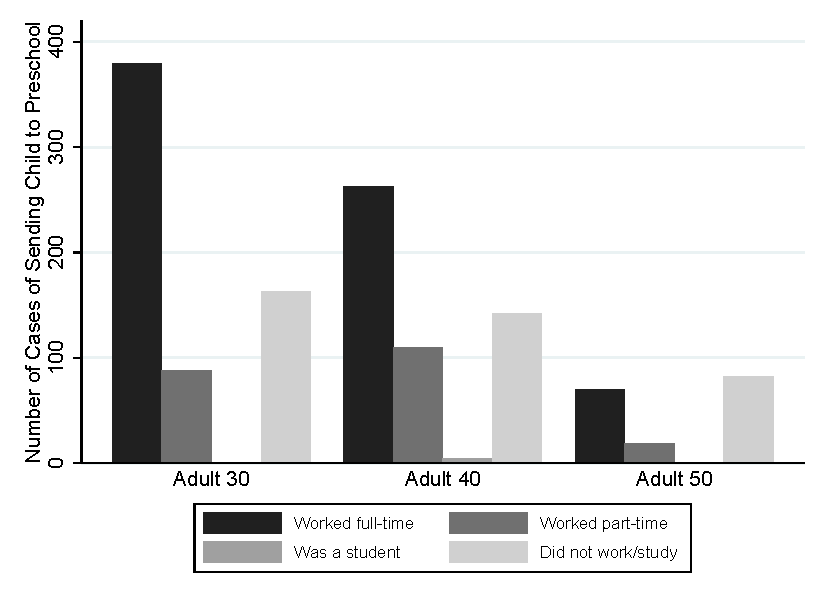
\includegraphics[scale=0.9]{../../../../output/image/bar_momworkpreschool_count.pdf}
\end{figure}

\begin{figure}[H] \caption{Mother's Employment and Preschool Choice, Percentage} \label{fig:m-emp-P-perc}
\centering
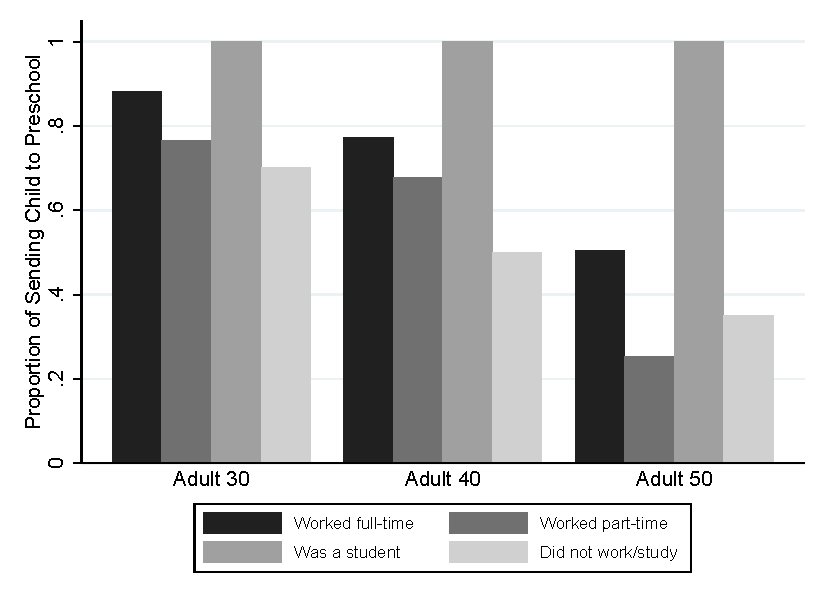
\includegraphics[scale=0.9]{../../../../output/image/bar_momworkpreschool_mean.pdf}
\end{figure}

Figure \ref{fig:m-emp-P-count} and \ref{fig:m-emp-P-perc} together show that more full-time working mothers enroll their children in preschool for age-30 cohort than age-50 cohort. It is also shown that significant proportion of mothers who did not work or study when the child was less than 6 years old sent their children to preschools, especially for the younger cohorts. 

One noticeable fact about the mothers of the age-50 cohort is that more than half of full-time working mothers did not send their children to any preschool. In order to see if they have alternative childcare option, we plot who the main caretaker during daytime was for this group in Figure \ref{fig:m-maincg}. 

\begin{figure}[H] \caption{Main Caregiver when Mother Worked Full-Time, Age-50 Cohort} \label{fig:m-maincg}
\centering
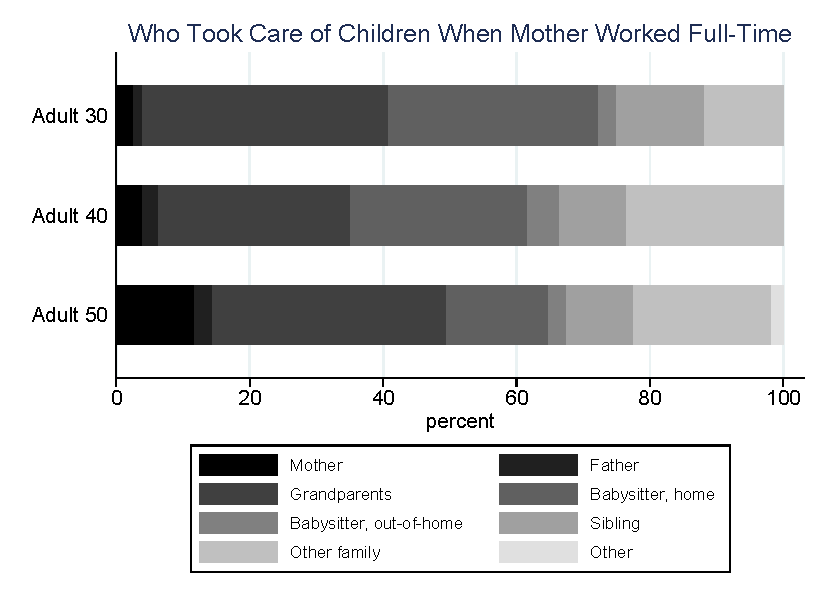
\includegraphics[scale=0.9]{../../../../output/image/bar_caregiver_momft.pdf}
\end{figure}


\section{Mother's Education and Preschool Choice}
We explore the relationship among mother's education level, mother's employment, and preschool choice to better understand the characteristics of working mothers and preschool decisions for each age-cohort. Figure \ref{fig:m-maxedu-work} shows the proportion of each maximum education level among working mothers (part-time and full-time). This shows that less educated mothers worked in age-50 cohort, but more educated mothers worked as we move to younger cohorts. 

\begin{figure}[H] \caption{Proportion of Each Max Education Level Among Working Mothers} \label{fig:m-maxedu-work}
\centering
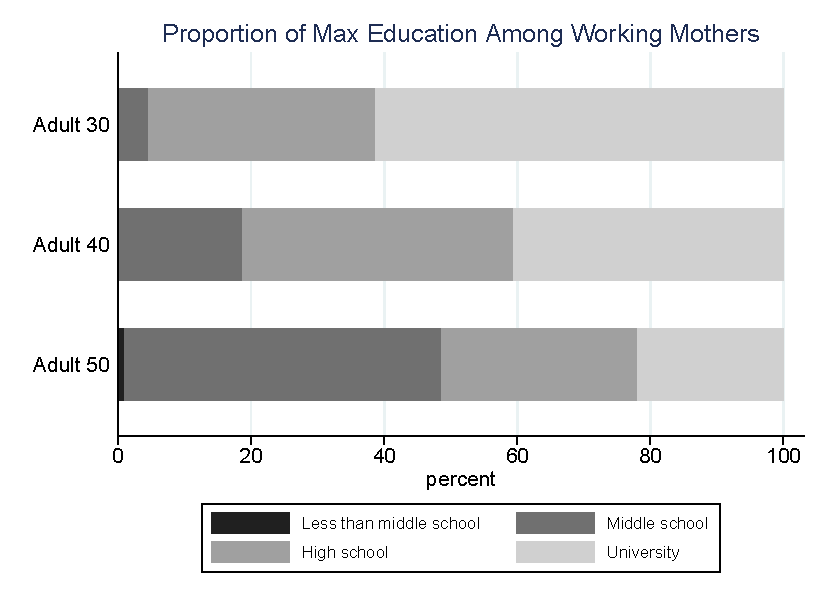
\includegraphics[scale=0.9]{../../../../output/image/bar_momeduwork.pdf}
\end{figure}

In order to investigate more into relationship among mother's education, working status, and preschool decision, we plot the density of mother's years of education for each age cohort for the following groups: \textbf{(1)} working mothers who sent their children to preschool, \textbf{(2)} working mothers who did not their children to preschool, \textbf{(3)} non-working mothers who sent their children to preschool, \textbf{(4)} non-working mothers who did not send their children to preschool.

\begin{figure}[H] \caption{Density of Mother's Years of Education for Each Work Status and Preschool Choice, Age-50 Cohort} \label{fig:density-medu-age50}
\centering
\includegraphics[scale=0.9]{../../../../output/image/kdensity_momeduworkmaterna_age50.pdf}
\end{figure}

\begin{figure}[H] \caption{Density of Mother's Years of Education for Each Work Status and Preschool Choice, Age-40 Cohort} \label{fig:density-medu-age40}
\centering
\includegraphics[scale=0.9]{../../../../output/image/kdensity_momeduworkmaterna_age40.pdf}
\end{figure}


\begin{figure}[H] \caption{Density of Mother's Years of Education for Each Work Status and Preschool Choice, Age-30 Cohort} \label{fig:density-medu-age30}
\centering
\includegraphics[scale=0.9]{../../../../output/image/kdensity_momeduworkmaterna_age30.pdf}
\end{figure}


Figure \ref{fig:density-medu-age50} shows that there is a very high concentration of low years of education among mothers who worked \textit{and} sent their children to preschool for age-50 cohort. In contrast, Figure \ref{fig:density-medu-age30} shows a high concentration of highly educated mothers among those who worked \textit{and} sent their children to preschool. This might imply that mothers of higher social status kept their children at home for age-50 cohort, but mothers of higher social status sent their children to preschools for age-30 cohort. 



\end{document}
